\documentclass[12pt,letterpaper]{article}
\usepackage{graphicx,textcomp}
\usepackage{natbib}
\usepackage{setspace}
\usepackage{fullpage}
\usepackage{color}
\usepackage[reqno]{amsmath}
\usepackage{amsthm}
\usepackage{fancyvrb}
\usepackage{amssymb,enumerate}
\usepackage[all]{xy}
\usepackage{endnotes}
\usepackage{lscape}
\newtheorem{com}{Comment}
\usepackage{float}
\usepackage{hyperref}
\newtheorem{lem} {Lemma}
\newtheorem{prop}{Proposition}
\newtheorem{thm}{Theorem}
\newtheorem{defn}{Definition}
\newtheorem{cor}{Corollary}
\newtheorem{obs}{Observation}
\usepackage[compact]{titlesec}
\usepackage{dcolumn}
\usepackage{tikz}
\usetikzlibrary{arrows}
\usepackage{multirow}
\usepackage{xcolor}
\newcolumntype{.}{D{.}{.}{-1}}
\newcolumntype{d}[1]{D{.}{.}{#1}}
\definecolor{light-gray}{gray}{0.65}
\usepackage{url}
\usepackage{listings}
\usepackage{color}

\definecolor{codegreen}{rgb}{0,0.6,0}
\definecolor{codegray}{rgb}{0.5,0.5,0.5}
\definecolor{codepurple}{rgb}{0.58,0,0.82}
\definecolor{backcolour}{rgb}{0.95,0.95,0.92}

\lstdefinestyle{mystyle}{
	backgroundcolor=\color{backcolour},   
	commentstyle=\color{codegreen},
	keywordstyle=\color{magenta},
	numberstyle=\tiny\color{codegray},
	stringstyle=\color{codepurple},
	basicstyle=\footnotesize,
	breakatwhitespace=false,         
	breaklines=true,                 
	captionpos=b,                    
	keepspaces=true,                 
	numbers=left,                    
	numbersep=5pt,                  
	showspaces=false,                
	showstringspaces=false,
	showtabs=false,                  
	tabsize=2
}
\lstset{style=mystyle}
\newcommand{\Sref}[1]{Section~\ref{#1}}
\newtheorem{hyp}{Hypothesis}

\title{Problem Set 1}
\date{Due: October 1, 2023}
\author{Valeriia Babaian}

\begin{document}
	\maketitle
	

	\vspace{1cm}
	\section*{Question 1 (40 points): Education}


\begin{enumerate}
	\item Find a 90\% confidence interval for the average student IQ in the school.\\
	\textit{Answer}: [93.95993; 102.92007].\\
	\vspace{.3cm}
	
	\lstinputlisting[language=R, firstline=41, lastline=52]{Babaian-PS01.R}  
	
	\vspace{.1cm}
	
	\item Next, the school counselor was curious  whether  the average student IQ in her school is higher than the average IQ score (100) among all the schools in the country.\\	\textit{Answer}: It is not higher:\\ 
		\vspace{.1cm}
	
	\lstinputlisting[language=R, firstline=57, lastline=58]{Babaian-PS01.R}  
	
	\vspace{.1cm}
	
	
	\noindent Using the same sample, conduct the appropriate hypothesis test with $\alpha=0.05$. \\	\textit{Answer}: Expectedly, the answer is the same as the average student IQ score in the given school was not greater than average IQ across the country on any of conventional levels of confidence.
		\vspace{.3cm}
	
	\lstinputlisting[language=R, firstline=60, lastline=61]{Babaian-PS01.R}  
	
	\vspace{.3cm}
\end{enumerate}

\newpage

	\section*{Question 2 (40 points): Political Economy}


\vspace{.5cm}
\noindent Explore the \texttt{expenditure} data set and import data into \texttt{R}.
\vspace{.2cm}
\lstinputlisting[language=R, firstline=67, lastline=68]{Babaian-PS01.R}  
\vspace{.2cm}
\begin{itemize}

\item
Please plot the relationships among \emph{Y}, \emph{X1}, \emph{X2}, and \emph{X3}? What are the correlations among them (you just need to describe the graph and the relationships among them)?
\vspace{.2cm}
\lstinputlisting[language=R, firstline=74, lastline=79]{Babaian-PS01.R}  
\vspace{.2cm} 

\vspace{.2cm}
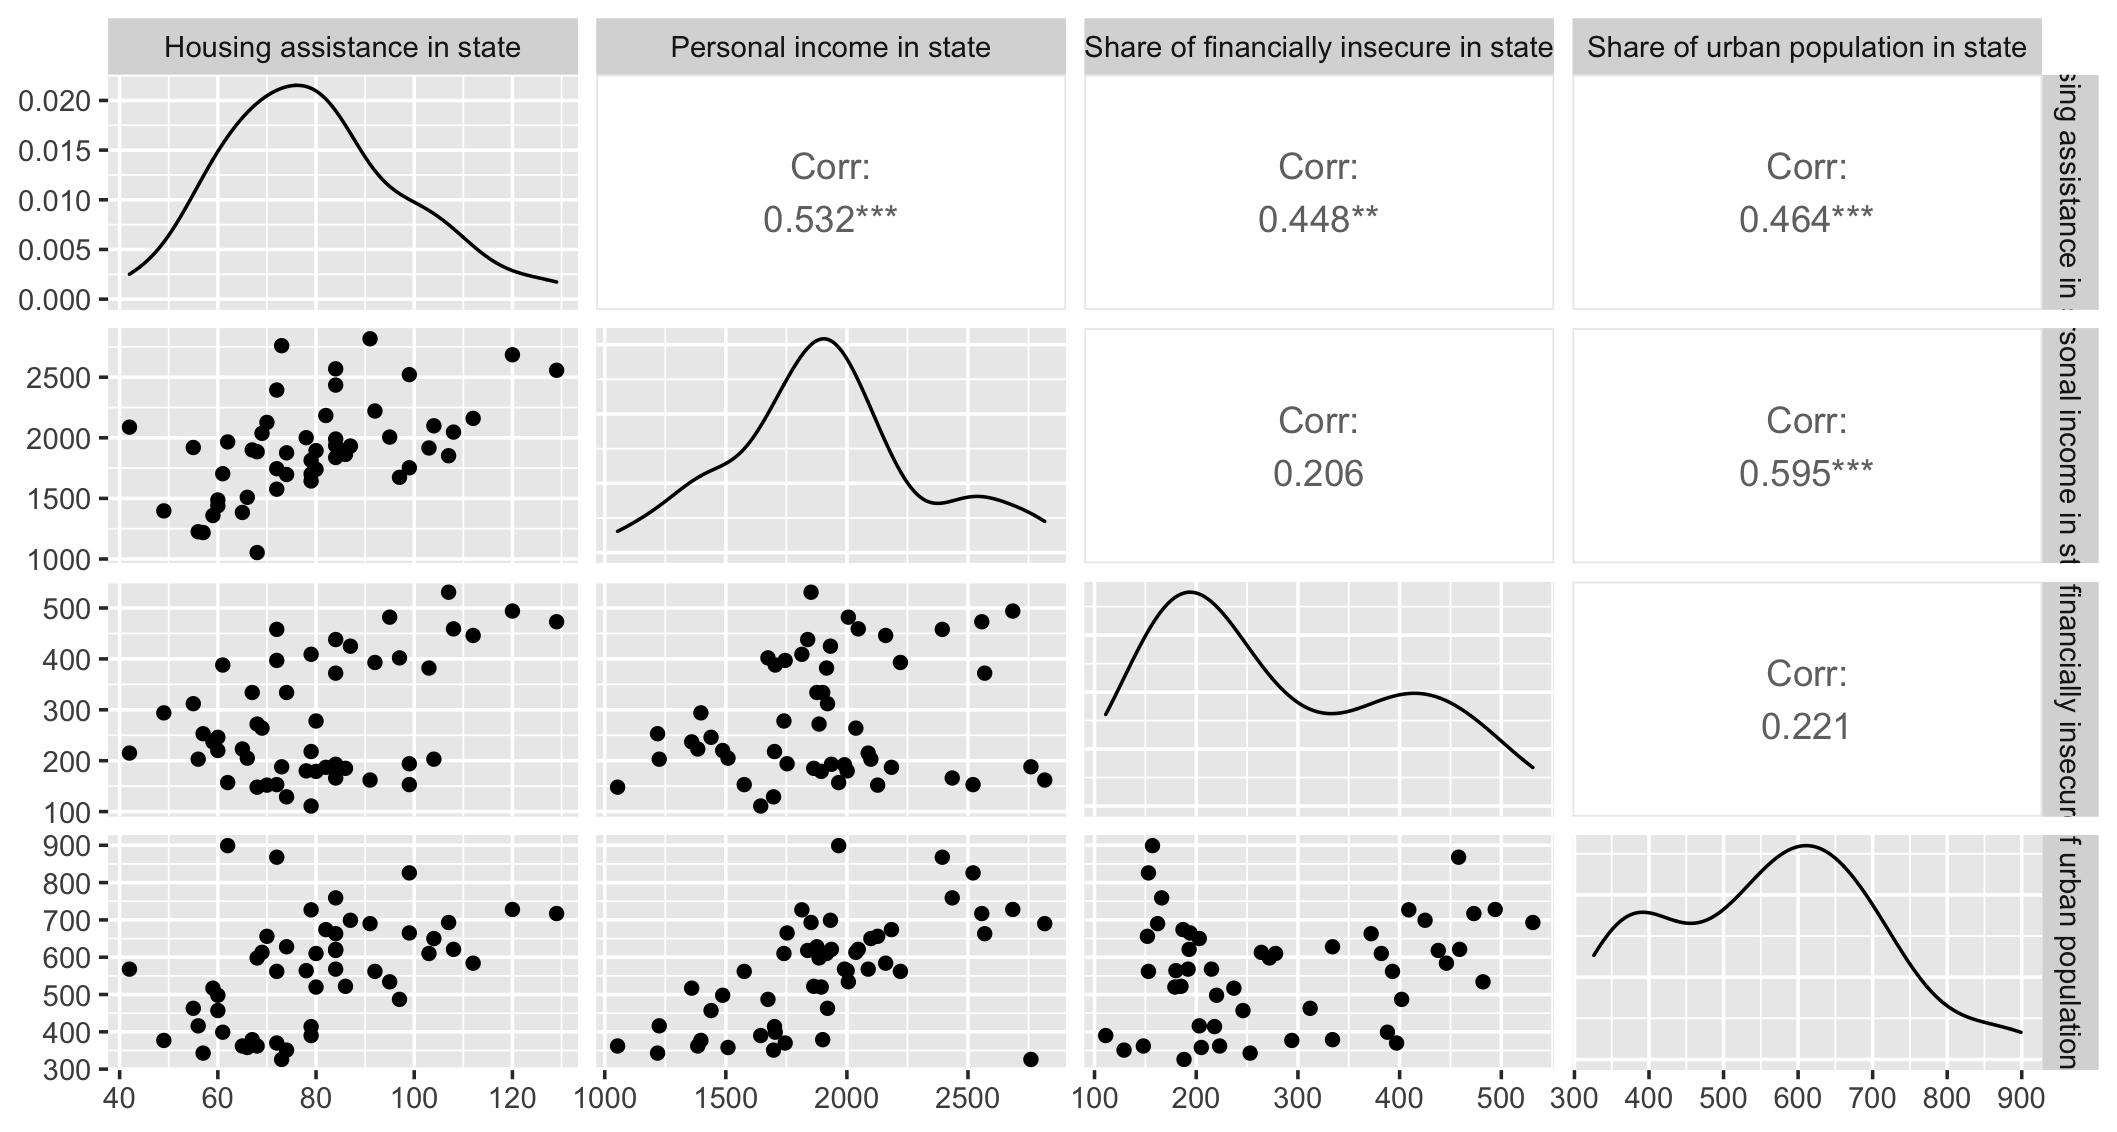
\includegraphics[width=\textwidth]{Babaian-plot1.png}
\vspace{.2cm}

According to the visualized relationships between all meaningful quantities in the data, the variables are positively related, but there are no strong correlations  between any of them. The upper-right part of the graphics proves this point.\\

\item
Please plot the relationship between \emph{Y} and \emph{Region}? On average, which region has the highest per capita expenditure on housing assistance?

\vspace{.2cm}
\lstinputlisting[language=R, firstline=87, lastline=94]{Babaian-PS01.R}  
\vspace{.2cm} 

\vspace{.2cm}
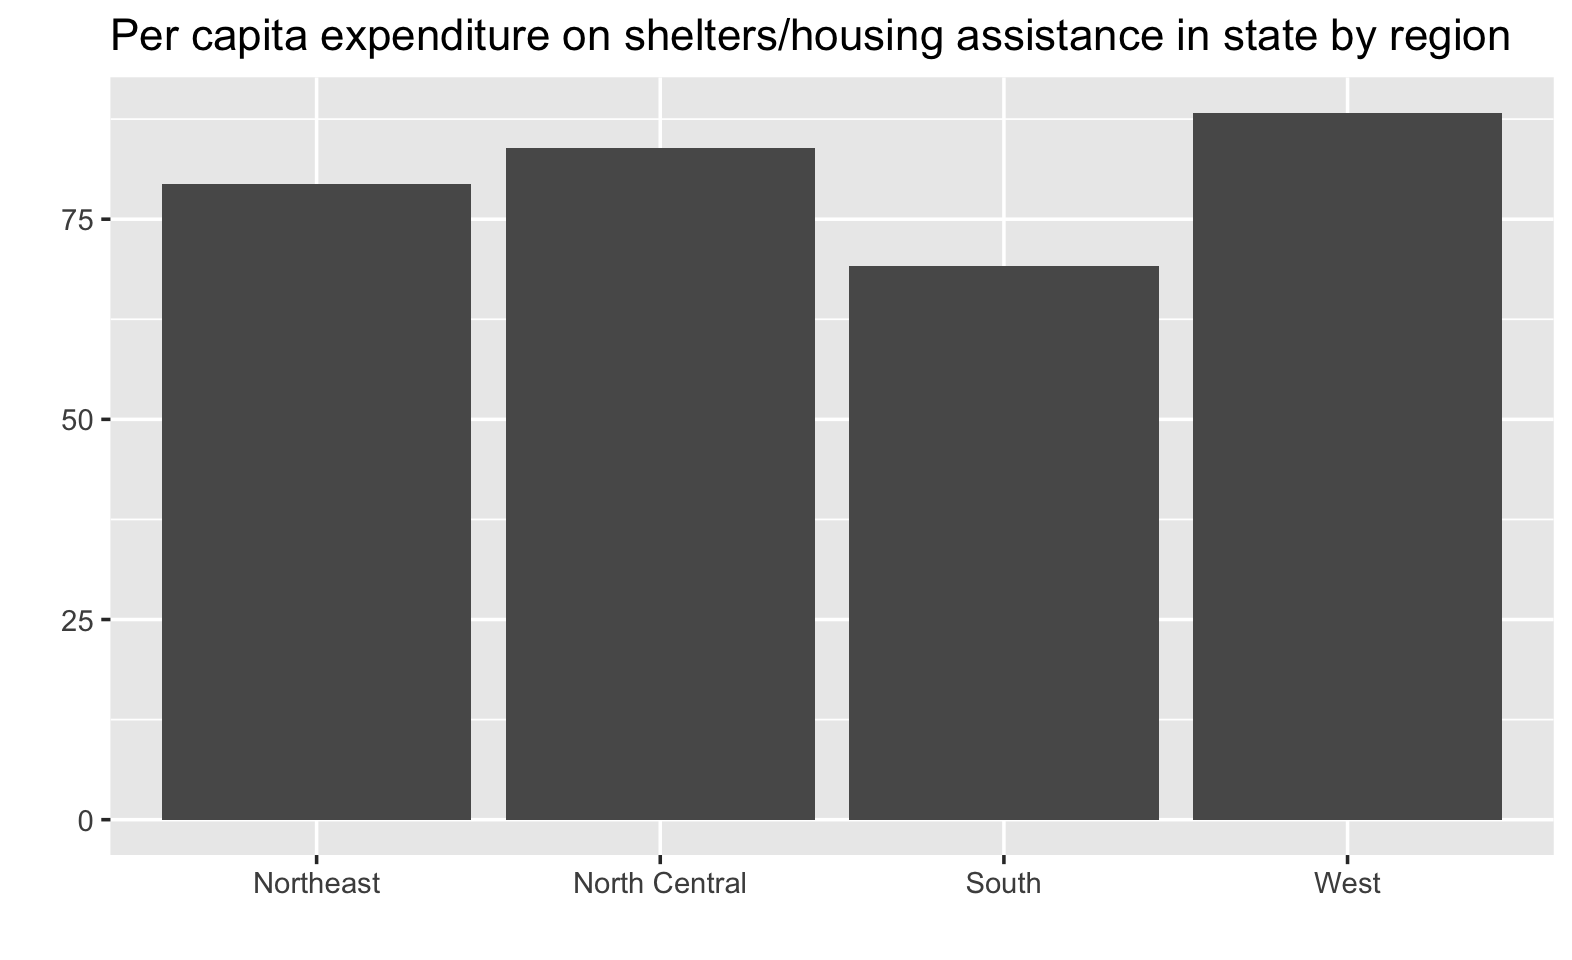
\includegraphics[width=\textwidth]{Babaian-plot2.png}
\vspace{.2cm}
The highest per capita expenditure on housing assistance is in the Western states.\\
\item
Please plot the relationship between \emph{Y} and \emph{X1}? Describe this graph and the relationship. Reproduce the above graph including one more variable \emph{Region} and display different regions with different types of symbols and colors.

\vspace{.2cm}
\lstinputlisting[language=R, firstline=98, lastline=101]{Babaian-PS01.R}  
\vspace{.2cm} 

\vspace{.2cm}
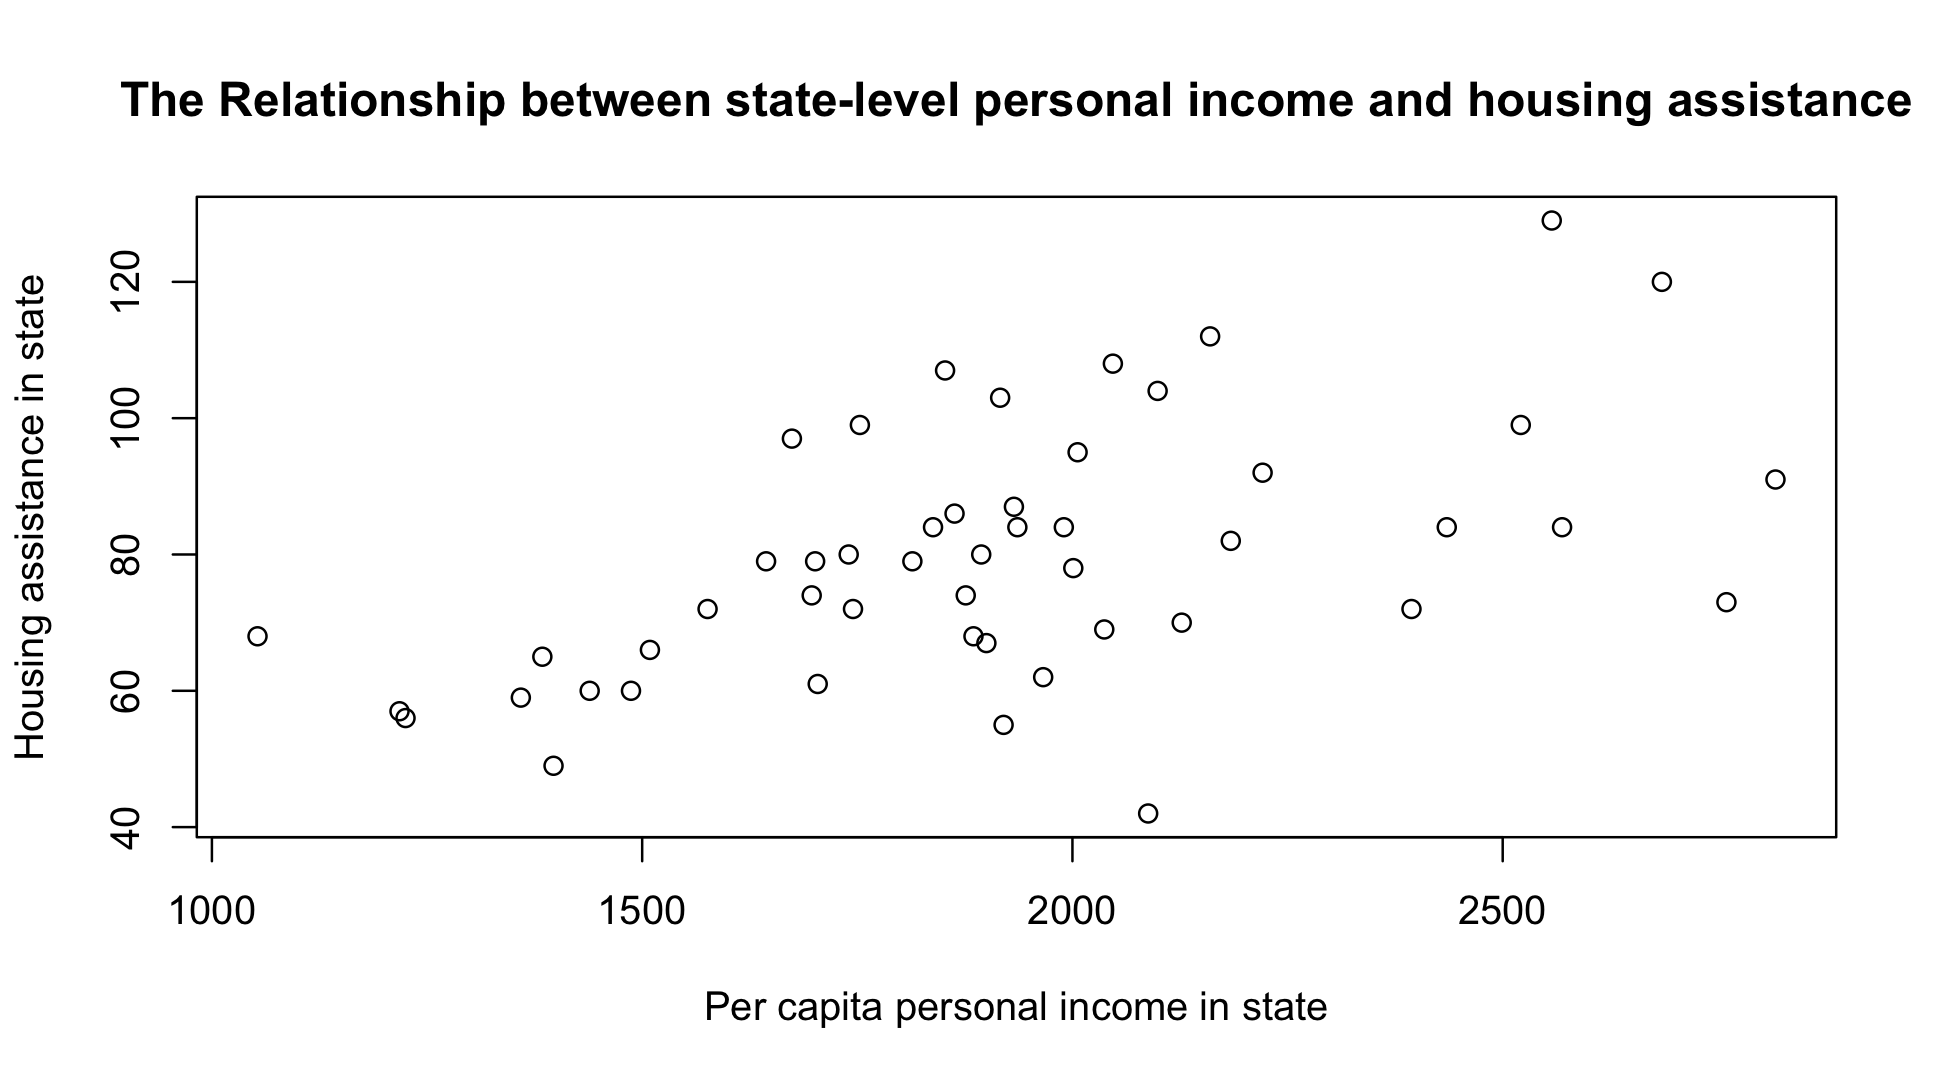
\includegraphics[width=\textwidth]{Babaian-plot3.png}
\vspace{.2cm}

There is a positive relationship between per capita personal income in state and its housing assistance expenditures, however, there is no strong correlation as there is a significant amount on deviations on both sides of the distributions.


\vspace{.2cm}
\lstinputlisting[language=R, firstline=109, lastline=116]{Babaian-PS01.R}  
\vspace{.2cm} 

\vspace{.2cm}
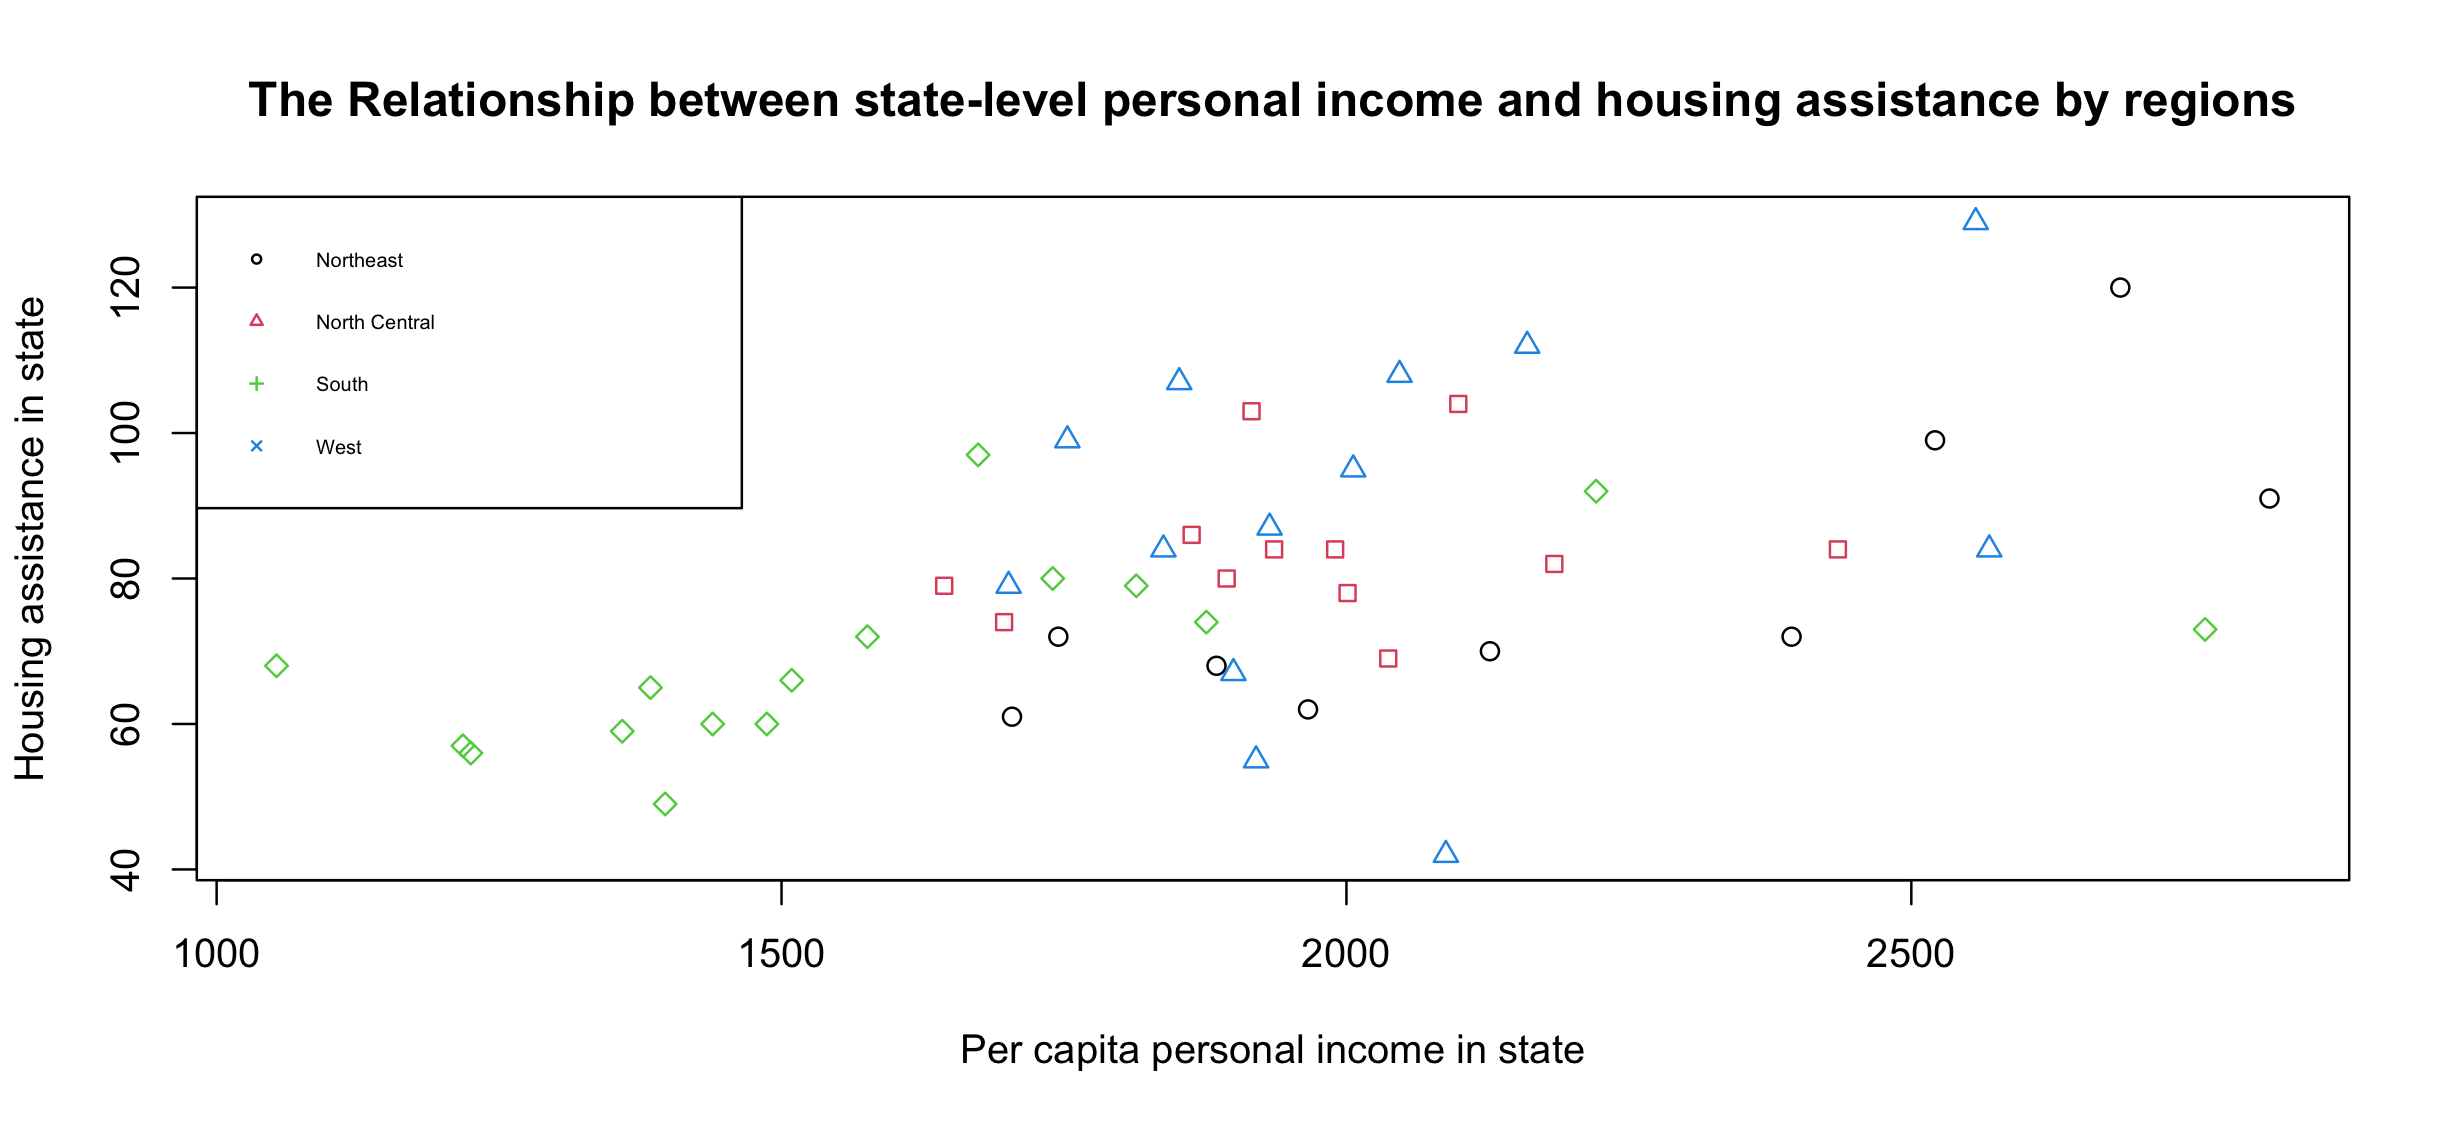
\includegraphics[width=\textwidth]{Babaian-plot4.png}
\vspace{.2cm}

\end{itemize}


\end{document}
